\section{Judas}
\label{met:Judas}

\subsection{Tools}
\label{met:Julia}

Created in 2009, first released in 2012 as part of a master thesis \cite{juliaMs} and further a doctoral thesis \cite{juliaPHD}, Julia is a high-performance, dynamically typed programming language with the goal of being a language ''fast and performant language like C, with syntax as simple as Python's, linear algebra extensions like Matlab, and statistics like R'' \cite{julia}. Like Python, Julia can be used in a script-like fashion through its \acrfull{repl}. Notebook-style programming has been a standard way for data analysts to write their code, and Jupyter notebooks also support Julia through the \texttt{IJulia.jl} package. Julia's fluent type system, accompanied by easy syntax, high performance, \acrshort{repl} tools, makes it a viable language for data science. We've previously discussed Julia in preliminary studies \cite{projthesis}. A full list of packages is detailed in Table in Appendix 

\subsection{Overview}
\label{met:judasoverview}

Judas, formerly known as Emerald from the project thesis \cite{projthesis}, is a Julia package we've created for internal use for members at \acrshort{cgf}. Our work started last fall when we saw a limitation of current applications at \acrshort{cgf} for loading \acrshort{das} data from local servers into programs to be able to process and further analyze these data. We wrote this package in Julia due to its high performance and members' familiarity with similar languages such as MatLab and Python. With Julia, we could draw strengths from its ecosystem and build systems to create an easy-to-use library with which members can familiarize themselves. We started with a simple Python program that read multiple \acrshort{hdf5} files storing \acrshort{das} data into data frames. We parallelized certain parts of the code from here and stored processed data in one memory-mapped file instead of loading large matrices into memory. This allowed us to work with more data at the same time, as well as decreasing the overall wall time and memory consumption.  
In this section, we will look at what changes have been made ever since, from improvements of existing code to new methods added and the availability of the library for members at \acrshort{cgf}. \\
We split our program into 4 parts: loading \acrshort{das} data from \acrshort{hdf5} files, signal processing, matrix operations, and utilities for plotting. A full overview of the file structure can be seen in Figure \ref{fig:judasoverview}.\\

\begin{figure}[!h]
    \centering
    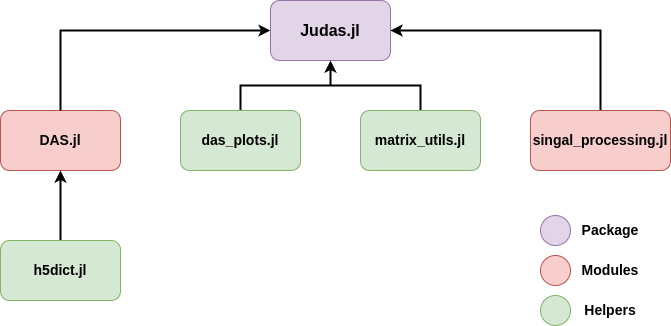
\includegraphics[scale=.5]{figures/judas_overview.png}
    \caption{File hierarchy in \texttt{Judas}}
    \label{fig:judasoverview}
\end{figure}

Figure \ref{fig:apiflow} shows which core functions have been changed or added to our program. Aside from these, all other utility functions are completely new. Compared to Emerald, Judas now contains more signal-processing methods and general utilities for plotting and loading files. Finding and loading files has also been improved or extended, aiming to reduce overall memory usage and processing time. \\
\begin{figure}[!h]
    \centering
    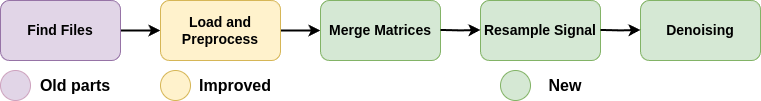
\includegraphics[scale=0.5]{figures/dataflow.png}
    \caption{Overview of both dataflow, as well as which functions have been improved since the project thesis \cite{projthesis}}
    \label{fig:apiflow}
\end{figure}
\subsection{Core Functionality}

\subsubsection{Finding \acrshort{das} files}
\label{met:finddasfiles}

The \texttt{find\_DAS\_files} function now allows for modifying the \acrfull{roi}, which determines which channels are included when loading the data. We introduced a \texttt{step} parameter for channel selection to enhance flexibility. As shown in Table \ref{tab:experiment_data}, every 4th sensor is stored in the original data. The \texttt{step} parameter allows users to adjust the interval between selected channels, effectively controlling the scale of \acrshort{das} data analysis. For instance, if the original channel distance was approximately \qty{4}{\meter}, setting \texttt{step} to 25 would result in loading data every \qty{100}{\meter}. This feature enables users to easily adapt the spatial resolution of their analysis to suit their specific needs.
The function returns the file paths of the \acrshort{hdf5} files, a list of channel indices to be loaded, and alternatively, which samples to load.

\subsubsection{Loading \acrshort{das} data}

The \lstinline{load_DAS_files} is the largest part of this , handling loading, metadata processing and numeric integration. 

The \texttt{DAS.jl} file has undergone massive changes. The primary modifications revolve around the \texttt{DASDataFrame} structure and parallelization. Previously, we wrote all \acrshort{das} data to a single memory-mapped binary file. This data is now distributed across multiple binary files, which can be loaded \textit{on-demand}. This new method optimizes data retrieval and storage efficiency. Furthermore, we handle some potential race conditions and use processes instead of threads to the parallelized section by synchronizing every process after they're done with local work. 


\lstinputlisting[label={code:parproc},caption=Parallel processing of \acrshort{das} signal matrices, language=Julia]{code/load_das_files.jl}

In code listing \ref{code:parproc}, we see how the function \texttt{process\_DAS\_chunk} is changed. By synchronizing the entire for-loop, we avoid problems of \acrshort{das} files not being processed before further loading them. Instead of directly writing to a binary file, we memory map the processed data before synchronizing the processed matrix with the file loaded in memory.

\textbf{Columnwise Cumulative Summation}

The decision to distribute the selected \acrshort{das} data across multiple files necessitated modifying a crucial function. Specifically, when the integrated parameter is enabled, a cumulative sum operation along the channel axis may be required. To address this requirement, we implemented a sequential operation denoted as \texttt{ccds!}, as illustrated in the following code snippet:

\lstinputlisting[label={code:ccds},caption=Columnwise Cumsum Delta Scaling, language=Julia]{code/ccds.jl}

The process begins with memory mapping of the submatrix $M_i$ from its respective file, where $i$ denotes the iteration index. Subsequently, the final row of the preceding matrix, represented as $prev_{i-1}$, is added to the initial row of the current submatrix: $M_i[1,:] \leftarrow M_i[1,:] + prev_{i-1}$. Following this, a column-wise cumulative sum operation is executed on $M_i$, such that $M_i[j,:] \leftarrow \sum_{k=1}^j M_i[k,:]$ for each column. The entire submatrix is then multiplied by the scaling factor $\Delta t$: $M_i \leftarrow \Delta t \cdot M_i$. Finally, the $prev_i$ variable is updated with the final row of the current submatrix to ensure continuity: $prev_i \leftarrow M_i[end,:]$. This $prev_i$ will be utilized in the subsequent iteration $i+1$, maintaining the cumulative nature of the operation across all submatrices. It is worth noting that $M_1$ has no previous row to add, and thus only computes the columnwise cumulative sum and gets scaled by $\Delta$t.

Our methodology enables the implementation of a column-wise cumulative sum operation across the entirety of the \acrshort{das} data, despite its distribution across multiple files. The iterative nature of this approach leverages Julia's compilation process; the initial function call triggers compilation, while subsequent calls utilize the compiled version, thereby enhancing computational efficiency.

The return type of the \texttt{load\_DAS\_files} function has also been slightly modified. In the previous implementation, a \texttt{DASDataFrame}, a vector of timestamps, was stored for each sample, which proved to be redundant. The revised approach leverages the inherent regularity of the sampling process. By storing only the initial timestamp and the sampling rate $F$, subsequent timestamps can be efficiently calculated using the following equation:
%
\begin{equation}
    t_{\text{now}} = t_{\text{start}} + MilliSecond(idx \times F \times 1000)
\end{equation}
%
This in-place calculation can be vectorized and broadcasted, improving computational efficiency. This modification reduces memory usage and maintains all essential temporal information required for subsequent data processing. Additionally, we store the number of rows in a single file, the number of files processed, and the \texttt{step} parameter we defined earlier to get an accurate channel distance after channel decimation.\\
\begin{figure}[!h]
\centering
\begin{subfigure}{.45\textwidth}
  \centering
  \lstinputlisting[language=Julia]{code/dasstructold.jl}
  \caption{Old \texttt{DASDataFrame} struct}
  \label{fig:olddasstc}
\end{subfigure}%
\hfill
\begin{subfigure}{.45\textwidth}
  \centering
  \lstinputlisting[language=Julia]{code/dasstruct.jl}
  \caption{New \texttt{DASDataFrame} struct}
  \label{fig:newdasstc}
\end{subfigure}
\caption{Comparison between previous and current version of the \texttt{DASDataFrame} struct}
\label{fig:dasstccmp}
\end{figure}
The entire \lstinline{load_DAS_files} is shown in the Appendix in Code Listing \ref{loaddas}.



\subsubsection{Parallel Resampling}


One effective method to reduce the memory consumption of \acrshort{das} signals is through resampling. Our approach utilizes the \texttt{SharedMatrix} datatype to allocate an output matrix $M_o$ that is accessible by all processes. Each process $p_i$ is assigned a subset of columns from the input matrix $M$ and performs the \texttt{resample} function (provided by the \texttt{DSP.jl} package) on its designated columns. For instance, given an initial sampling frequency of \qty{2000}{\hertz} and a target frequency of \qty{100}{\hertz}, we can achieve a 20-fold reduction in memory consumption. This process is implemented in our \texttt{das\_resample} function, as demonstrated in Listing \ref{code:parres}:

\lstinputlisting[label={code:parres}, caption=Parallel Columnwise Matrix Resample, language=Julia]{code/parallel_resample.jl}

\clearpage
\subsubsection{Denoising \acrshort{das} signals}

\lstinputlisting[caption=Denoise function, language=Julia, label={code:denoise}]{code/denoise.jl}

The last addition to \texttt{Judas.jl} is the \texttt{denoise} function as seen in Code Listing \ref{code:denoise}. It combines tapering and digital filtering techniques, producing an efficient algorithm for \acrshort{das} signal denoising. Some of the more important aspects include: 

\begin{itemize}
    \item A Tukey window, as described in Section \ref{dsp:tukey}, to mitigate edge effects.
    \item Cutoff frequencies are normalized by the Nyquist frequency \cite{schmogrow2012nyquist}.
    \item The \texttt{filtfilt} function applies a zero-phase filter, preserving the original signal. This filter type is, by default, set as a bandpass. 
\end{itemize}

\clearpage
\subsection{General Usage and Distribution}

Through these functionalities, users may find and load data, perform channel decimation, and denoise the signals. To illustrate the ease of use, the following code listing \ref{code:judas} showcases its simplicity and how users can easily use it alongside other packages. \\

\lstinputlisting[label={code:judas}, caption=This codesnippet showcases a typical usecase for Judas, language=Julia]{code/judas_usage.jl}

To run this code, we can either add processes within the program with the \texttt{addprocs(amount::Int)} function or start Julia in a distributed environment, as shown below.

\begin{lstlisting}[style=shellcommand, language=bash, label={code:judasrun}]
(*@\textcolor{promptcolor}{\$}@*) julia -p 4 run.jl
\end{lstlisting}

In addition to the methods we've described in detail, multiple helper methods exist for plotting and reading/writing \acrshort{das} data. \texttt{Judas.jl} v1.1.0 is currently available for use for members at \acrshort{cgf}. 

